\documentclass[../../main.tex]{subfiles}

\graphicspath{{../../image/}{../../figure/}}

\begin{document}

\section{判别分类器}\label{section:ch05-判别分类器}

对于二分类情况，我们已经看到，针对指数族分布中多种类-条件概率密度$p(\boldsymbol{x}\mid C_k)$的选择问题，$C_1$类的后验概率可以写成作用于$\boldsymbol{x}$的线性函数的 logistic sigmoid 函数。同样，对于多分类情况，$C_k$类的后验概率由作用于$\boldsymbol{x}$的线性函数的 softmax 变换给出。对于类-条件概率密度$p(\boldsymbol{x}\mid C_k)$的具体选择，我们首先使用最大似然法确定密度参数和类的先验概率$p(C_k)$，然后使用 Bayes 定理求出类的后验概率。此为生成式模型的一个例子，我们可以利用该模型，通过从边缘分布$p(\boldsymbol{x})$或任何类-条件概率密度$p(\boldsymbol{x}\mid C_k)$中取$\boldsymbol{x}$值而生成合成数据。

不过，还有一种方法是明确使用广义线性模型的函数形式并通过最大似然法直接确定其参数。在这种直接方法中，我们将似然函数（由条件分布$p(C_k\mid\boldsymbol{x})$定义）最大化，此为一种判别概率建模形式。我们很快就能看到，判别法的一个优点是，需要确定的可学习参数通常较少。此外，判别法还可以提高预测性能，尤其当类-条件概率密度的假定形式与真实分布的近似程度较低时。

\subsection{激活函数}\label{subsection:ch05-激活函数}

在线性回归（参见\cref{section:ch04-线性回归}）中，模型预测值$y(\boldsymbol{x},\boldsymbol{w})$由参数的线性函数给出：

\begin{align}
  y(\boldsymbol{x},\boldsymbol{w})=\boldsymbol{w}^{\mathsf{T}}\boldsymbol{x}+w_0
  \label{align:ch05-线性回归模型}
\end{align}

它给出了范围为$(-\infty,\infty)$的连续值输出。然而，对于分类问题，我们希望预测离散类标签，或者更一般地说，预测$(0,1)$范围内的后验概率。为此，我们考虑对这一模型进行泛化——用非线性函数$f(\cdot)$对$\boldsymbol{w}$和$w_0$的线性函数进行转换，从而得到

\begin{align}
  y(\boldsymbol{x},\boldsymbol{w})=f\left(\boldsymbol{w}^{\mathsf{T}}\boldsymbol{x}+w_0\right)
  \label{align:ch05-激活模型}
\end{align}

\begin{definition}[激活函数与连接函数]\label{definition:ch05-激活函数}
在\eqref{align:ch05-激活模型}中，$f(\cdot)$在机器学习文献中称为激活函数（activation function），它的反函数$f^{-1}(\cdot)$在统计学文献中则称为连接函数（link function）。
\end{definition}

% SUPPLEMENT: parent=definition:ch05-激活函数; kind=motivation; location=紧随其后的 remark（重构新增）
\begin{remark}（重构新增）
激活函数的作用是把无界的线性输出$\boldsymbol{w}^{\mathsf{T}}\boldsymbol{x}+w_0$压缩到后验概率所需的区间$(0,1)$内；连接函数则是从概率出发的同一对象：它把均值$y$映回线性预激活。两者互为反函数，因此“选激活函数”与“选连接函数”是同一件事的两种说法。$f$必须是单调的，否则同一个$y$可能对应多个预激活，决策面将不再是单个超平面。$f$的值域必须是$(0,1)$的子集，否则输出不能解释为概率；若允许端点，则需额外约定。注意$f$的非线性不改变决策面的形状：决策面仍由$\boldsymbol{w}^{\mathsf{T}}\boldsymbol{x}+w_0=\text{常数}$给出，因为$f$单调（见下面的讨论）。
\end{remark}

决策面对应于$y(\boldsymbol{x})=\text{常数}$，因此$\boldsymbol{w}^{\mathsf{T}}\boldsymbol{x}=\text{常数}$，决策面是$\boldsymbol{x}$的线性函数，即使函数$f(\cdot)$是非线性的。因此，\eqref{align:ch05-激活模型}描述的这一类模型名为广义线性模型（McCullagh and Nelder, 1989）。

\begin{definition}[广义线性模型]\label{definition:ch05-广义线性模型}
若模型对输入$\boldsymbol{x}$的依赖只通过线性组合$\boldsymbol{w}^{\mathsf{T}}\boldsymbol{x}+w_0$体现，而输出由非线性（单调）函数$f$作用于该线性组合得到，即具有\eqref{align:ch05-激活模型}的形式，则称它为广义线性模型（generalized linear model）。
\end{definition}

% SUPPLEMENT: parent=definition:ch05-广义线性模型; kind=motivation; location=紧随其后的 remark（重构新增）
\begin{remark}（重构新增）
“广义线性”中的“线性”指线性预激活，“广义”指允许$f$非线性；因此它既不同于线性回归（$f$为恒等映射），也不同于一般非线性模型（$f$的自变量不是线性的）。这种结构带来两个后果：其一，决策面仍是超平面（因为$f$单调，$y$的等值面对应$\boldsymbol{w}^{\mathsf{T}}\boldsymbol{x}+w_0$的等值面）；其二，对参数的依赖是非线性的，故不能像线性最小二乘那样用一次线性方程求解，必须用迭代方法（见\cref{subsection:ch05-logistic回归}）。条件“$f$单调”不是定义的字面要求，而是使决策面为超平面所必需的；若$f$不单调，$y=\text{常数}$可能对应多个超平面。
\end{remark}

然而，与用于回归的模型相比，由于非线性函数$f(\cdot)$的存在，这些模型的参数不再是线性的。这将导致比线性回归模型更复杂的分析和计算特性。不过，与更为灵活的非线性模型（后续章节将对它们展开研究）相比，这些模型仍然相对简单。

\subsection{固定基函数}\label{subsection:ch05-固定基函数}

前面介绍了直接使用原始输入向量$\boldsymbol{x}$的分类模型。不过，如果我们首先使用基函数$\boldsymbol{\phi}(\boldsymbol{x})$的向量对输入进行固定的非线性变换，那么所有算法都同样适用。如\cref{figure:ch05-基函数特征}所示，由此产生的决策边界在特征空间$\boldsymbol{\phi}$中是线性的，与原始观测空间$\boldsymbol{x}$中的非线性决策边界相对应。特征空间$\boldsymbol{\phi}$中可线性分离的类在原始观测空间$\boldsymbol{x}$中不必线性可分。

\begin{definition}[固定基函数模型]\label{definition:ch05-固定基函数模型}
设$\boldsymbol{\phi}(\boldsymbol{x})=(\phi_1(\boldsymbol{x}),\cdots,\phi_M(\boldsymbol{x}))^{\mathsf{T}}$是给定的、不随数据改变的非线性变换。若分类模型只通过线性组合$\boldsymbol{w}^{\mathsf{T}}\boldsymbol{\phi}(\boldsymbol{x})+w_0$使用输入，则称它为固定基函数模型（fixed basis function model），$\phi_i$称为基函数。
\end{definition}

\begin{figure}[htbp]
  \centering
  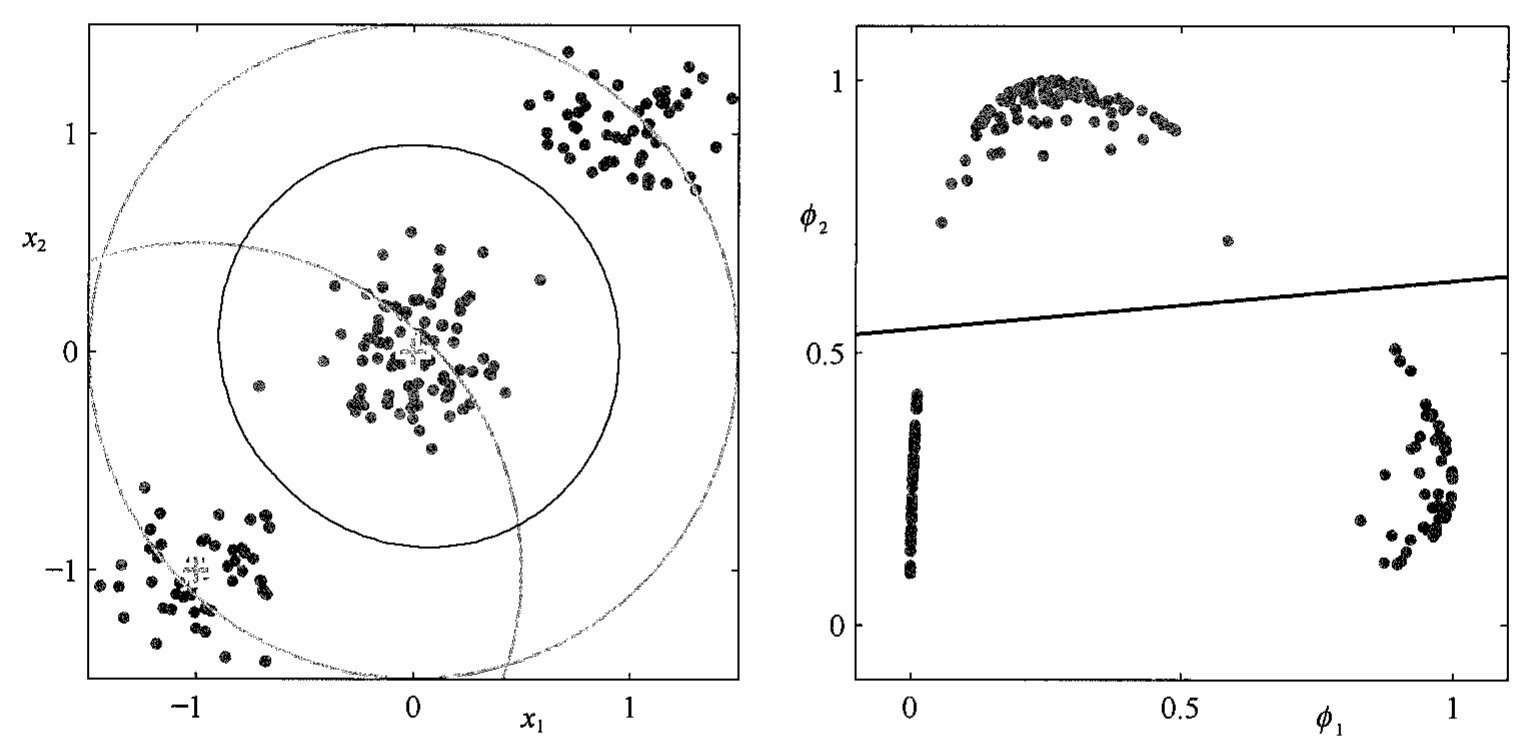
\includegraphics[width=0.96\textwidth]{ch05-fig5-15-basis-features.png}
  \caption{非线性基函数在线性分类模型中发挥作用的示意图。左图展示了原始输入空间$(x_1,x_2)$以及两个类（标记为红色和蓝色）中的数据点。此空间中定义了两个“Gauss”基函数$\phi_1(\boldsymbol{x})$和$\phi_2(\boldsymbol{x})$，中心用绿色十字表示，轮廓用绿色圆圈表示。右图展示了相应的特征空间$(\phi_1,\phi_2)$，以及由\cref{subsection:ch05-logistic回归}所述形式的 logistic 回归模型得到的线性决策边界。这与原始输入空间中的非线性决策边界相对应，如左图中的黑色曲线所示}
  \label{figure:ch05-基函数特征}
\end{figure}

请注意，在线性回归模型中，有一个基函数通常设为常数，例如$\phi_0(\boldsymbol{x})=1$，因此相应的参数$w_0$起到偏置的作用。

% SUPPLEMENT: parent=definition:ch05-固定基函数模型; kind=motivation; location=紧随其后的 remark（重构新增）
\begin{remark}（重构新增）
固定基函数模型的意义在于：线性分类算法的全部理论（线性决策面、凸决策区域、最大似然）都可以原样搬到一个新的特征空间中，从而在原始空间中产生非线性边界。代价是基函数的个数$M$与形式必须事先选定：若$M$太小则表达能力不足，若$M$太大则参数增多、容易过拟合。\cref{figure:ch05-基函数特征}中，左图用两个径向基函数把二维输入映到二维特征空间，右图中的直线在左图中对应一条闭曲线，正好把中心的一类与外围的另一类分开。条件“基函数固定、不随数据改变”是关键：一旦让基函数依赖于数据或参数，模型就不再是广义线性的，而成为后续章节讨论的神经网络。
\end{remark}

在许多实际问题中，类-条件概率密度$p(\boldsymbol{x}\mid C_k)$在$\boldsymbol{x}$空间中存在明显的重叠。这相当于后验概率$p(C_k\mid\boldsymbol{x})$，至少对于$\boldsymbol{x}$的某些值，后验概率$p(C_k\mid\boldsymbol{x})$不是0或1。在这种情况下，通过对后验概率进行精确建模并应用标准决策理论（参见\cref{section:ch05-决策理论}），便可得到最优解。请注意，非线性变换$\phi_k(\boldsymbol{x})$并不能消除这种重叠，尽管它们可以增加重叠程度，或在原始观测空间中不存在重叠的地方产生重叠。非线性的适当选择可以使后验概率建模过程变得更容易。然而，这种固定的基函数模型有很大的局限性（参见\cref{section:ch06-固定基函数的局限性}），在后续章节中，我们将通过让基函数适应数据来解决这些问题。

\subsection{logistic 回归}\label{subsection:ch05-logistic回归}

首先考虑二分类问题。在\cref{section:ch05-生成分类器}关于生成方法的讨论中，我们看到了在一般假设条件下，$C_1$的后验概率可以写成作用于特征空间$\boldsymbol{\phi}$的线性函数的 logistic sigmoid 函数，从而得到

\begin{align}
  p(C_1\mid\boldsymbol{\phi})=y(\boldsymbol{\phi})=\sigma\left(\boldsymbol{w}^{\mathsf{T}}\boldsymbol{\phi}\right)
  \label{align:ch05-logistic模型}
\end{align}

其中$p(C_2\mid\boldsymbol{\phi})=1-p(C_1\mid\boldsymbol{\phi})$由\cref{definition:ch05-logistic-sigmoid}定义的 logistic sigmoid 函数给出。

\begin{definition}[logistic 回归模型]\label{definition:ch05-logistic回归}
若二分类模型的后验概率取\eqref{align:ch05-logistic模型}的形式，其中$\sigma$为 logistic sigmoid 函数、$\boldsymbol{\phi}=\boldsymbol{\phi}(\boldsymbol{x})$为特征向量，则称该模型为 logistic 回归（logistic regression）模型。
\end{definition}

% SUPPLEMENT: parent=definition:ch05-logistic回归; kind=motivation; location=紧随其后的 remark（重构新增）
\begin{remark}（重构新增）
名称中的“回归”是历史遗留：它来自统计学中对二值响应变量做广义线性建模的传统，但模型输出的是类后验概率，因此它实际上是一个分类模型，而不是连续变量模型。这一名称容易引起误解，阅读时应以“输出为$(0,1)$内的概率、决策面为超平面”为准。模型的可调参数是$\boldsymbol{w}$（若含偏置则增加一个分量），共$M$个（$M$为特征维数）。与生成式方法相比，logistic 回归不假设$\boldsymbol{\phi}$的分布，因此对类-条件密度的假设错误不敏感；但它也不能生成数据，不能直接用于离群值检测。
\end{remark}

对于$M$维特征空间$\boldsymbol{\phi}$，该模型有$M$个可调参数。相比之下，如果我们使用最大似然法拟合 Gauss 类-条件概率密度，那么我们将使用$2M$个参数表示均值，并使用$M(M+1)/2$个参数表示（共享）协方差矩阵。再加上类的先验概率$p(C_1)$，总共有$M(M+5)/2+1$个参数。与 logistic 回归模型中参数数量与$M$成线性关系不同，该模型的参数数量随$M$呈二次增长。对于较大的$M$值，直接使用 logistic 回归模型有明显的优势。

下面我们使用最大似然法确定 logistic 回归模型的参数。为此，我们将利用 logistic sigmoid 函数的导数，它可以方便地用 sigmoid 函数本身来表示（见\cref{exercise:ch05-18}）：

\begin{align}
  \frac{\mathrm{d}\sigma}{\mathrm{d}a}=\sigma(1-\sigma)
  \label{align:ch05-sigmoid导数}
\end{align}

\begin{proposition}[logistic sigmoid 函数的导数]\label{proposition:ch05-sigmoid导数}
设$\sigma(a)=1/(1+\exp(-a))$，则$\sigma$可微且$\sigma'(a)=\sigma(a)\bigl(1-\sigma(a)\bigr)$对一切$a\in\mathbb{R}$成立。
\end{proposition}

\begin{proof}
（重构新增）由$\sigma(a)=(1+e^{-a})^{-1}$，用链式法则：
\begin{align}
  \sigma'(a)=-(1+e^{-a})^{-2}\cdot(-e^{-a})=\frac{e^{-a}}{(1+e^{-a})^{2}}=\frac{1}{1+e^{-a}}\cdot\frac{e^{-a}}{1+e^{-a}}=\sigma(a)\bigl(1-\sigma(a)\bigr)
\end{align}
其中最后一个等号用了$1-\sigma(a)=e^{-a}/(1+e^{-a})$。由于$e^{-a}>0$，右端恒为正，故$\sigma$严格单调递增。
\end{proof}

% SUPPLEMENT: parent=proposition:ch05-sigmoid导数; kind=motivation; location=紧随其后的 remark（重构新增）
\begin{remark}（重构新增）
$\sigma'=\sigma(1-\sigma)$是 logistic 回归计算上便利的根本原因：交叉熵的导数中会出现因子$y_n(1-y_n)$，正好被这个恒等式消去，从而得到\cref{proposition:ch05-交叉熵梯度}中“误差乘特征”的简洁形式。该恒等式也说明$\sigma'\leqslant 1/4$（因为$\sigma(1-\sigma)$在$\sigma=1/2$处取最大值$1/4$），因此$\sigma$是 Lipschitz 常数为$1/4$的压缩映射，这保证了梯度下降的稳定性。注意$\sigma'$在$|a|$很大时趋于0，这就是“梯度饱和”现象的来源。
\end{remark}

对于数据集$\{\boldsymbol{\phi}_n,t_n\}$，其中$\boldsymbol{\phi}_n=\boldsymbol{\phi}(\boldsymbol{x}_n)$，且$t_n\in\{0,1\}$，$n=1,\cdots,N$。似然函数可写成

\begin{align}
  p(\boldsymbol{t}\mid\boldsymbol{w})=\prod_{n=1}^{N}y_n^{t_n}(1-y_n)^{1-t_n}
  \label{align:ch05-logistic似然}
\end{align}

其中$\boldsymbol{t}=(t_1,\cdots,t_N)^{\mathsf{T}}$，且$y_n=p(C_1\mid\boldsymbol{\phi}_n)$。按照惯例，我们可以通过取似然的负对数来定义误差函数，从而得到交叉熵（cross-entropy）误差函数：

\begin{align}
  E(\boldsymbol{w})=-\ln p(\boldsymbol{t}\mid\boldsymbol{w})=-\sum_{n=1}^{N}\bigl\{t_n\ln y_n+(1-t_n)\ln(1-y_n)\bigr\}
  \label{align:ch05-交叉熵}
\end{align}

其中，$y_n=\sigma(a_n)$且$a_n=\boldsymbol{w}^{\mathsf{T}}\boldsymbol{\phi}_n$。利用误差函数关于$\boldsymbol{w}$的梯度，可得（见\cref{exercise:ch05-19}）

\begin{align}
  \nabla E(\boldsymbol{w})=\sum_{n=1}^{N}(y_n-t_n)\boldsymbol{\phi}_n
  \label{align:ch05-交叉熵梯度式}
\end{align}

\begin{proposition}[交叉熵误差的梯度]\label{proposition:ch05-交叉熵梯度}
设$E(\boldsymbol{w})$由\eqref{align:ch05-交叉熵}定义，$y_n=\sigma(\boldsymbol{w}^{\mathsf{T}}\boldsymbol{\phi}_n)$。则$E$可微，且其梯度由\eqref{align:ch05-交叉熵梯度式}给出。
\end{proposition}

\begin{proof}
（重构新增）记$a_n=\boldsymbol{w}^{\mathsf{T}}\boldsymbol{\phi}_n$。由\cref{proposition:ch05-sigmoid导数}，
\begin{align}
  \frac{\partial E}{\partial a_n}=-\frac{t_n}{y_n}y_n(1-y_n)+\frac{1-t_n}{1-y_n}y_n(1-y_n)=-t_n(1-y_n)+(1-t_n)y_n=y_n-t_n
\end{align}
再由$\partial a_n/\partial\boldsymbol{w}=\boldsymbol{\phi}_n$与链式法则，$\nabla E=\sum_n(\partial E/\partial a_n)\boldsymbol{\phi}_n=\sum_n(y_n-t_n)\boldsymbol{\phi}_n$，即\eqref{align:ch05-交叉熵梯度式}。
\end{proof}

% SUPPLEMENT: parent=proposition:ch05-交叉熵梯度; kind=motivation; location=紧随其后的 remark（重构新增）
\begin{remark}（重构新增）
命题中的推导显示：sigmoid 的导数因子$y_n(1-y_n)$在分子与分母中同时出现而被约去，这正是 logistic 回归“梯度形式简单”的原因。若把交叉熵换成平方误差$E=\frac12\sum(y_n-t_n)^2$，则梯度中会残留因子$y_n(1-y_n)$，当$y_n$接近0或1时梯度消失，收敛变慢，这就是分类问题不宜用平方误差的理论依据。梯度的形式$\sum_n(y_n-t_n)\boldsymbol{\phi}_n$与线性回归中平方和误差的梯度形式完全相同（见\cref{align:ch04-似然梯度}），差别只在于$y_n$是$\boldsymbol{w}$的非线性函数。$\nabla E=0$等价于$\sum_n y_n\boldsymbol{\phi}_n=\sum_n t_n\boldsymbol{\phi}_n$，即“预测的充分统计量等于观测的充分统计量”。
\end{remark}

其中，我们使用了\eqref{align:ch05-sigmoid导数}。你可以看到，涉及 logistic sigmoid 导数的因子已被消去，从而简化了对数似然梯度的形式。具体来说，数据点$n$对梯度的贡献由目标值与模型预测值之间的“误差”$(y_n-t_n)$乘以$\boldsymbol{\phi}_n$给出。此外，通过与\cref{align:ch04-似然梯度}进行比较，我们发现这与线性回归模型的平方和误差函数梯度的形式完全相同。

最大似然解（参见\cref{subsection:ch04-最大似然}）对应于$\nabla E(\boldsymbol{w})=0$。然而，从\eqref{align:ch05-交叉熵梯度式}中可以看出，由于$y(\cdot)$的非线性，这不再对应于线性方程组，因此没有闭式解。

\begin{remark}（重构新增）
“没有闭式解”的确切含义是：驻点方程$\sum_n\bigl(\sigma(\boldsymbol{w}^{\mathsf{T}}\boldsymbol{\phi}_n)-t_n\bigr)\boldsymbol{\phi}_n=\boldsymbol{0}$中，未知量$\boldsymbol{w}$出现在 sigmoid 的自变量内，因而它不是关于$\boldsymbol{w}$的线性方程组，不能像\eqref{align:ch05-最小二乘解}那样用一次矩阵求逆写出解。这并不意味着解不存在（凸性保证解存在，见\cref{proposition:ch05-交叉熵凸性}），而是说不存在由有限次四则运算与初等函数组成的通用表达式。数值上可用 Newton 法（即 IRLS）或梯度下降求解。
\end{remark}

求最大似然解的一种方法是使用随机梯度下降法（参见\cref{chapter:ch07-梯度下降}），其中$\nabla E_n$是\eqref{align:ch05-交叉熵梯度式}右侧的第$n$项。随机梯度下降法是训练高度非线性神经网络（后续章节将展开讨论）的主要方法。然而，最大似然方程只是“略微”非线性的。事实上，由\eqref{align:ch05-logistic模型}定义的模型，其误差函数\eqref{align:ch05-交叉熵}是参数的凸函数，这使得误差函数可以通过一种称为迭代重加权最小二乘法（Iterative Reweighted Least Squares, IRLS）的简单算法来最小化（Bishop, 2006）。然而，这很难泛化到更复杂的模型，如深度神经网络。

\begin{proposition}[交叉熵误差的凸性]\label{proposition:ch05-交叉熵凸性}
设$E(\boldsymbol{w})$由\eqref{align:ch05-交叉熵}定义。则$E$是$\boldsymbol{w}$的凸函数；若$\{\boldsymbol{\phi}_n\}$张成整个参数空间，则$E$还是严格凸的。
\end{proposition}

\begin{proof}
（重构新增）由$y_n=\sigma(a_n)$，把\eqref{align:ch05-交叉熵}改写为
\begin{align}
  E(\boldsymbol{w})=\sum_{n=1}^{N}\left\{\ln\left(1+e^{a_n}\right)-t_na_n\right\}
\end{align}
其中用到$-\ln\sigma(a)=\ln(1+e^{-a})$与$-\ln(1-\sigma(a))=\ln(1+e^{a})$。对$a_n$求二阶导：$\dfrac{\mathrm{d}^{2}}{\mathrm{d}a_n^{2}}\ln(1+e^{a_n})=\sigma(a_n)\bigl(1-\sigma(a_n)\bigr)\geqslant 0$，而$-t_na_n$关于$a_n$是线性的，二阶导为零。于是
\begin{align}
  \nabla^{2}E(\boldsymbol{w})=\sum_{n=1}^{N}\sigma(a_n)\bigl(1-\sigma(a_n)\bigr)\boldsymbol{\phi}_n\boldsymbol{\phi}_n^{\mathsf{T}}\succeq\boldsymbol{0}
\end{align}
即 Hessian 半正定，故$E$凸。若$\{\boldsymbol{\phi}_n\}$张成整个空间，则对任意$\boldsymbol{v}\neq\boldsymbol{0}$存在$n$使$\boldsymbol{v}^{\mathsf{T}}\boldsymbol{\phi}_n\neq0$；又$0<\sigma(1-\sigma)$，故$\boldsymbol{v}^{\mathsf{T}}\nabla^{2}E\boldsymbol{v}>0$，Hessian 正定，$E$严格凸。
\end{proof}

% SUPPLEMENT: parent=proposition:ch05-交叉熵凸性; kind=motivation; location=紧随其后的 remark（重构新增）
\begin{remark}（重构新增）
凸性保证任何局部极小都是全局极小，因此梯度下降不会陷入局部最优；严格凸性还保证极小点唯一（若存在）。证明的关键恒等式是“logistic 损失的二阶导等于方差$\sigma(1-\sigma)$”，这也是 IRLS 中“权重”的来源：每步用当前$y_n(1-y_n)$作为样本权重做加权最小二乘。注意凸性是关于$\boldsymbol{w}$的，而不是关于$y$的；$\boldsymbol{\phi}_n$固定时结论成立，若基函数依赖于$\boldsymbol{w}$（如神经网络），凸性一般不再成立，这正是深度网络优化更困难的原因之一。
\end{remark}

请注意，对于线性可分的数据集，最大似然法可能会表现出严重的过拟合。这是因为当$\sigma=0.5$（相当于$\boldsymbol{w}^{\mathsf{T}}\boldsymbol{\phi}=0$）所对应的超平面将两个类分开，且$\boldsymbol{w}$的大小趋于无穷时，就会出现最大似然解。在这种情况下，logistic sigmoid 函数在特征空间中变得无限陡峭，相当于一个单位阶跃函数，因此来自每个类的每个训练点都被赋予一个后验概率$p(C_k\mid\boldsymbol{x})=1$（见\cref{exercise:ch05-20}）。此外，这样的解通常是连续的，因为任何分离超平面在训练点处都会产生相同的后验概率。最大似然法无法提供最优解，在实践中找到那个解将取决于优化算法的选择和参数是如何初始化的。注意，只要训练数据集是线性可分的，即使数据点的数量相比模型中参数的数量很大，问题也会出现。在误差函数中加入正则化项（参见\cref{chapter:ch09-正则化}）可以避免奇异解。

\begin{proposition}[线性可分数据的最大似然问题无有限解]\label{proposition:ch05-线性可分最大似然}
设训练集线性可分，即存在$\boldsymbol{w}^{*}$使$t_n=1$时$(\boldsymbol{w}^{*})^{\mathsf{T}}\boldsymbol{\phi}_n>0$、$t_n=0$时$(\boldsymbol{w}^{*})^{\mathsf{T}}\boldsymbol{\phi}_n<0$。则似然\eqref{align:ch05-logistic似然}在$\boldsymbol{w}$上的上确界为1，但任何有限的$\boldsymbol{w}$都取不到该值；特别地，最大似然问题没有有限解，且沿$\boldsymbol{w}=c\boldsymbol{w}^{*}$（$c\to\infty$）的任一方向都趋向该上确界。
\end{proposition}

\begin{proof}
（重构新增）对任意有限的$\boldsymbol{w}$与任意$n$，$a_n=\boldsymbol{w}^{\mathsf{T}}\boldsymbol{\phi}_n$有限，故$y_n=\sigma(a_n)\in(0,1)$且$1-y_n\in(0,1)$。于是\eqref{align:ch05-logistic似然}的每个因子都在$(0,1)$内，乘积严格小于1，即任何有限$\boldsymbol{w}$处的似然都小于1。

另一方面，令$\boldsymbol{w}=c\boldsymbol{w}^{*}$，$c>0$。对$t_n=1$的数据点，$a_n=c(\boldsymbol{w}^{*})^{\mathsf{T}}\boldsymbol{\phi}_n\to+\infty$，故$y_n=\sigma(a_n)\to1$；对$t_n=0$的数据点，$a_n\to-\infty$，故$1-y_n=\sigma(-a_n)\to1$。于是\eqref{align:ch05-logistic似然}的每个因子都趋于1，有限个因子的乘积也趋于1（$N$固定）。因此似然的上确界为1且不可达，最大似然解不存在；又因该论证对任何使数据分开的方向$\boldsymbol{w}^{*}$都成立，故这样的方向构成一个连续统。
\end{proof}

% SUPPLEMENT: parent=proposition:ch05-线性可分最大似然; kind=motivation; location=紧随其后的 remark（重构新增）
\begin{remark}（重构新增）
命题说明“过拟合”在这里表现为参数发散而非某个有限的坏解：模型对训练点的后验概率都趋于1，训练误差为零，但$\lVert\boldsymbol{w}\rVert\to\infty$使决策面在特征空间中变得极陡，任何靠近训练点的测试点都会被赋予接近0或1的概率，泛化性能由$\boldsymbol{w}$的初始值与优化路径决定。条件“线性可分”不可去掉：若数据不可分，则最优$\boldsymbol{w}$有限，似然的最大值在驻点处取到（由\cref{proposition:ch05-交叉熵凸性}，该驻点唯一）。加入正则化项$\lambda\lVert\boldsymbol{w}\rVert^{2}$（见\cref{chapter:ch09-正则化}）后，目标函数变为强凸，即使数据线性可分也存在唯一有限解。
\end{remark}

\subsection{多类 logistic 回归}\label{subsection:ch05-多类logistic回归}

在讨论用于多分类的生成式模型（参见\cref{section:ch05-生成分类器}）时，我们已经看到，对于指数族分布，后验概率是由作用于特征变量的线性函数的 softmax 变换给出的，于是有

\begin{align}
  p(C_k\mid\boldsymbol{\phi})=y_k(\boldsymbol{\phi})=\frac{\exp(a_k)}{\sum_j\exp(a_j)}
  \label{align:ch05-多类后验}
\end{align}

其中，预激活$a_k$为

\begin{align}
  a_k=\boldsymbol{w}_k^{\mathsf{T}}\boldsymbol{\phi}
  \label{align:ch05-多类线性预激活}
\end{align}

此处，我们使用最大似然法分别确定了类-条件概率密度和类的先验，然后使用 Bayes 定理找到了相应的后验概率，从而隐式地确定了参数$\{\boldsymbol{w}_k\}$。下面考虑使用最大似然法直接确定参数$\{\boldsymbol{w}_k\}$。为此，我们需要$y_k$相对于所有预激活$a_j$的导数，计算公式为（见\cref{exercise:ch05-21}）

\begin{align}
  \frac{\partial y_k}{\partial a_j}=y_k\left(I_{kj}-y_j\right)
  \label{align:ch05-softmax导数式}
\end{align}

其中，$I_{kj}$是单位矩阵的元素。

\begin{proposition}[softmax 函数的导数]\label{proposition:ch05-softmax导数}
设$y_k=e^{a_k}/\sum_j e^{a_j}$，$k=1,\cdots,K$。则$\dfrac{\partial y_k}{\partial a_j}=y_k(I_{kj}-y_j)$，其中$I_{kj}$为$K\times K$单位矩阵的元素。
\end{proposition}

\begin{proof}
（重构新增）记$S=\sum_j e^{a_j}$，则$y_k=e^{a_k}/S$。当$j\neq k$时，$e^{a_k}$与$S$对$a_j$的偏导分别为0与$e^{a_j}$，故
\begin{align}
  \frac{\partial y_k}{\partial a_j}=-\frac{e^{a_k}e^{a_j}}{S^{2}}=-y_ky_j=y_k(0-y_j)
\end{align}
当$j=k$时，$e^{a_k}$对$a_k$的偏导为$e^{a_k}$，故
\begin{align}
  \frac{\partial y_k}{\partial a_k}=\frac{e^{a_k}S-e^{a_k}e^{a_k}}{S^{2}}=y_k-y_k^{2}=y_k(1-y_k)
\end{align}
两式合并即得$\partial y_k/\partial a_j=y_k(I_{kj}-y_j)$。
\end{proof}

% SUPPLEMENT: parent=proposition:ch05-softmax导数; kind=motivation; location=紧随其后的 remark（重构新增）
\begin{remark}（重构新增）
该导数矩阵$\partial y/\partial a$是 softmax 的 Jacobian，它是半正定的（对任意$\boldsymbol{v}$，$\boldsymbol{v}^{\mathsf{T}}\partial y/\partial a\,\boldsymbol{v}=\sum_k y_k v_k^{2}-(\sum_k y_kv_k)^{2}\geqslant0$，即方差非负）。$K=2$时令$a=a_1-a_2$，该式退化为$\sigma'(a)=\sigma(1-\sigma)$，与\cref{proposition:ch05-sigmoid导数}一致。由于 softmax 具有平移不变性，Jacobian 的零空间至少包含全1向量，这与多类模型参数的冗余一致（把所有权重同时加上同一个向量不改变模型）。
\end{remark}

接下来让我们写下似然函数。使用1-of-$K$编码方案最容易实现这一目标，在这种编码方案下，属于$C_k$类的$\boldsymbol{\phi}_n$的目标向量$\boldsymbol{t}_n$是一个二进制向量，除元素$k$等于1外，其他元素均为0。似然函数为

\begin{align}
  p(\boldsymbol{T}\mid\boldsymbol{w}_1,\cdots,\boldsymbol{w}_K)=\prod_{n=1}^{N}\prod_{k=1}^{K}p(C_k\mid\boldsymbol{\phi}_n)^{t_{nk}}=\prod_{n=1}^{N}\prod_{k=1}^{K}y_{nk}^{t_{nk}}
  \label{align:ch05-多类似然}
\end{align}

其中$y_{nk}=y_k(\boldsymbol{\phi}_n)$，且$\boldsymbol{T}$是一个包含$N\times K$个目标变量的矩阵，其中的元素为$t_{nk}$。取负对数可得

\begin{align}
  E(\boldsymbol{w}_1,\cdots,\boldsymbol{w}_K)=-\ln p(\boldsymbol{T}\mid\boldsymbol{w}_1,\cdots,\boldsymbol{w}_K)=-\sum_{n=1}^{N}\sum_{k=1}^{K}t_{nk}\ln y_{nk}
  \label{align:ch05-多类交叉熵}
\end{align}

此为多分类问题的交叉熵误差函数。

下面求误差函数相对于参数向量$\boldsymbol{w}_j$的梯度。利用\eqref{align:ch05-softmax导数式}对 softmax 函数求导可得（见\cref{exercise:ch05-22}）

\begin{align}
  \nabla_{\boldsymbol{w}_j}E(\boldsymbol{w}_1,\cdots,\boldsymbol{w}_K)=\sum_{n=1}^{N}\left(y_{nj}-t_{nj}\right)\boldsymbol{\phi}_n
  \label{align:ch05-多类梯度式}
\end{align}

\begin{proposition}[多类交叉熵误差的梯度]\label{proposition:ch05-多类梯度}
设$E$由\eqref{align:ch05-多类交叉熵}定义，$y_{nk}$由\eqref{align:ch05-多类后验}与\eqref{align:ch05-多类线性预激活}给出，且每个$\boldsymbol{t}_n$满足$\sum_k t_{nk}=1$。则$E$关于$\boldsymbol{w}_j$的梯度由\eqref{align:ch05-多类梯度式}给出。
\end{proposition}

\begin{proof}
（重构新增）由链式法则与\eqref{align:ch05-softmax导数式}，
\begin{align}
  \frac{\partial E}{\partial a_{nj}}=-\sum_{k=1}^{K}\frac{t_{nk}}{y_{nk}}\frac{\partial y_{nk}}{\partial a_{nj}}=-\sum_{k=1}^{K}\frac{t_{nk}}{y_{nk}}y_{nk}\left(I_{kj}-y_{nj}\right)=-\sum_{k=1}^{K}t_{nk}I_{kj}+y_{nj}\sum_{k=1}^{K}t_{nk}=-t_{nj}+y_{nj}
\end{align}
其中最后一步用了$\sum_k t_{nk}=1$。又$a_{nj}=\boldsymbol{w}_j^{\mathsf{T}}\boldsymbol{\phi}_n$，故$\partial a_{nj}/\partial\boldsymbol{w}_j=\boldsymbol{\phi}_n$，于是$\nabla_{\boldsymbol{w}_j}E=\sum_n(y_{nj}-t_{nj})\boldsymbol{\phi}_n$。
\end{proof}

% SUPPLEMENT: parent=proposition:ch05-多类梯度; kind=motivation; location=紧随其后的 remark（重构新增）
\begin{remark}（重构新增）
命题与二分类的\cref{proposition:ch05-交叉熵梯度}形式完全一致，这不是巧合：softmax 与交叉熵的配对使 sigmoid 的导数因子被约去，从而每个参数只“感受”到本类的误差。条件$\sum_k t_{nk}=1$在推导中用于把$\sum_k t_{nk}I_{kj}$化为$t_{nj}$；对1-of-$K$编码它自动成立，若目标不是1-of-$K$（例如软标签），该条件仍成立但$t_{nk}$可以取$(0,1)$内的值。多类模型中参数存在冗余：把每个$\boldsymbol{w}_j$同时加上同一向量$\boldsymbol{v}$不改变任何$a_{nj}$的差，故最优解不唯一；实践中通常靠正则化或固定某个参考类来消除冗余。原书\eqref{align:ch05-权重梯度}左端对$w_{ij}$求导，而右端误差的下标写作$k$，这是同一对象的两种记法（$w_{ij}$把第$i$个基函数连接到第$k$个输出单元），阅读时以右端的$k$为准。
\end{remark}

其中，我们利用了$\sum_k t_{nk}=1$。同样，我们可以利用随机梯度下降法（参见\cref{chapter:ch07-梯度下降}）来优化参数。

我们再次发现，梯度的形式与线性模型的平方和误差函数和 logistic 回归模型的交叉熵误差函数的形式相同，即误差$(y_{nj}-t_{nj})$与基函数激活度$\boldsymbol{\phi}_n$的乘积。我们稍后将探讨更普遍的例子（参见\cref{subsection:ch05-规范连接函数}）。

线性分类模型可表示为单层神经网络，如\cref{figure:ch05-单层网络}所示。如果我们使用误差函数相对于权重$w_{ik}$的导数（以便将基函数$\phi_i(\boldsymbol{x})$与输出单元$t_k$连接起来），则可以得出

\begin{align}
  \frac{\partial E(\boldsymbol{w}_1,\cdots,\boldsymbol{w}_K)}{\partial w_{ij}}=\sum_{n=1}^{N}\left(y_{nk}-t_{nk}\right)\phi_i(\boldsymbol{x}_n)
  \label{align:ch05-权重梯度}
\end{align}

\begin{figure}[htbp]
  \centering
  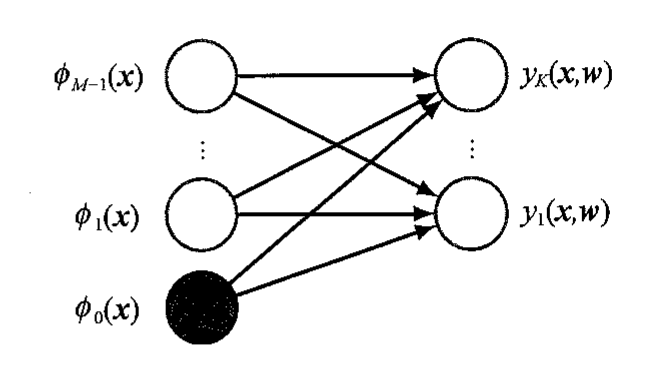
\includegraphics[width=0.55\textwidth]{ch05-fig5-16-network.png}
  \caption{将线性分类模型表示为具有单层连接的神经网络。每个基函数由一个节点表示，实心节点表示“偏置”基函数$\phi_0$，而每个输出$y_1,\cdots,y_K$也由一个节点表示。节点之间的连接代表相应的权重和偏置参数}
  \label{figure:ch05-单层网络}
\end{figure}

与\cref{figure:ch05-单层网络}相比，我们可以看到，对于每个数据点$n$，梯度的形式是权重链路输入端的基函数输出与输出端“误差”$(y_{nk}-t_{nk})$的乘积。

\subsection{probit 回归}\label{subsection:ch05-probit回归}

我们已经看到，对于各种类-条件分布，得到的后验类率（posterior class probability）是由作用于特征变量线性函数的 logistic（或 softmax）变换给出的。然而，并不是类-条件概率密度的所有选择都能为后验概率生成如此简单的形式，这表明也许值得探索其他类型的判别概率模型。在广义线性模型的框架内，再次考虑二分类情况，得到

\begin{align}
  p(t=1\mid a)=f(a)
  \label{align:ch05-阈值模型}
\end{align}

其中，$a=\boldsymbol{w}^{\mathsf{T}}\boldsymbol{\phi}$且$f(\cdot)$为激活函数。

激发替代连接函数的一种方法是使用噪声阈值模型（noisy threshold model）。对于每个输入$\boldsymbol{\phi}_n$，评估$a_n=\boldsymbol{w}^{\mathsf{T}}\boldsymbol{\phi}_n$，然后根据以下公式设定目标值：

\begin{align}
  \begin{cases}
    t_n=1, & a_n\geqslant\theta\\
    t_n=0, & \text{其他}
  \end{cases}
  \label{align:ch05-阈值判定}
\end{align}

\begin{definition}[噪声阈值模型]\label{definition:ch05-噪声阈值模型}
设每个输入$\boldsymbol{\phi}_n$对应一个线性预激活$a_n=\boldsymbol{w}^{\mathsf{T}}\boldsymbol{\phi}_n$，并设阈值$\theta$是一个随机变量，其概率密度为$p(\theta)$。若目标值按\eqref{align:ch05-阈值判定}设定，即当$a_n\geqslant\theta$时取$t_n=1$、否则取$t_n=0$，则称该模型为噪声阈值模型（noisy threshold model）。
\end{definition}

% SUPPLEMENT: parent=definition:ch05-噪声阈值模型; kind=motivation; location=紧随其后的 remark（重构新增）
\begin{remark}（重构新增）
噪声阈值模型的动机是：真实的类标签往往由某个未观测的阈值决定，而阈值本身带有随机性（测量误差、个体差异等），把它建模为随机变量就得到一条平滑的激活函数。阈值$\theta$的分布不同，得到的$f$就不同：$\theta$取 logistic 分布时得到 logistic sigmoid，取 Gauss 分布时得到 probit（见\cref{definition:ch05-probit函数}）。条件“$\theta$与$\boldsymbol{\phi}_n$独立”是隐含的，否则$f$还要依赖于$\boldsymbol{\phi}_n$，模型不再是广义线性的。\eqref{align:ch05-阈值判定}中$a_n=\theta$的取法（大于等于还是大于）只影响零概率事件，不影响下面的积分表达式。
\end{remark}

如果$\theta$值来自概率密度$p(\theta)$，那么相应的激活函数将由累积分布函数（cumulative distribution function）给出：

\begin{align}
  f(a)=\int_{-\infty}^{a}p(\theta)\,\mathrm{d}\theta
  \label{align:ch05-累积分布激活}
\end{align}

如\cref{figure:ch05-噪声阈值}所示。

\begin{proposition}[噪声阈值模型的激活函数]\label{proposition:ch05-噪声阈值激活}
设$\theta$的概率密度为$p(\theta)$，目标值按\eqref{align:ch05-阈值判定}设定，且$\theta$与$\boldsymbol{\phi}$独立。则$p(t=1\mid a)=f(a)$，其中$f$由\eqref{align:ch05-累积分布激活}给出。
\end{proposition}

\begin{proof}
（重构新增）由全概率公式并对$\theta$的边缘分布积分，
\begin{align}
  p(t=1\mid a)=\int_{-\infty}^{\infty}p(t=1\mid a,\theta)\,p(\theta)\,\mathrm{d}\theta
\end{align}
由\eqref{align:ch05-阈值判定}，给定$\theta$时$t=1$当且仅当$a\geqslant\theta$，故$p(t=1\mid a,\theta)=\mathbb{I}\{\theta\leqslant a\}$。于是
\begin{align}
  p(t=1\mid a)=\int_{-\infty}^{\infty}\mathbb{I}\{\theta\leqslant a\}\,p(\theta)\,\mathrm{d}\theta=\int_{-\infty}^{a}p(\theta)\,\mathrm{d}\theta=f(a)
\end{align}
即\eqref{align:ch05-累积分布激活}。
\end{proof}

% SUPPLEMENT: parent=proposition:ch05-噪声阈值激活; kind=motivation; location=紧随其后的 remark（重构新增）
\begin{remark}（重构新增）
命题说明：任何概率分布函数都可以充当激活函数，因此“选择激活函数”等价于“选择阈值的噪声分布”。这解释了为什么 probit 与 logistic 都合理：它们分别对应 Gauss 噪声与 logistic 噪声。累积分布函数自动满足单调、值域为$[0,1]$，这正是\cref{definition:ch05-激活函数}所要求的。若$p(\theta)$关于0对称，则$f(0)=1/2$，决策面过原点（在增广空间中）。
\end{remark}

\begin{figure}[htbp]
  \centering
  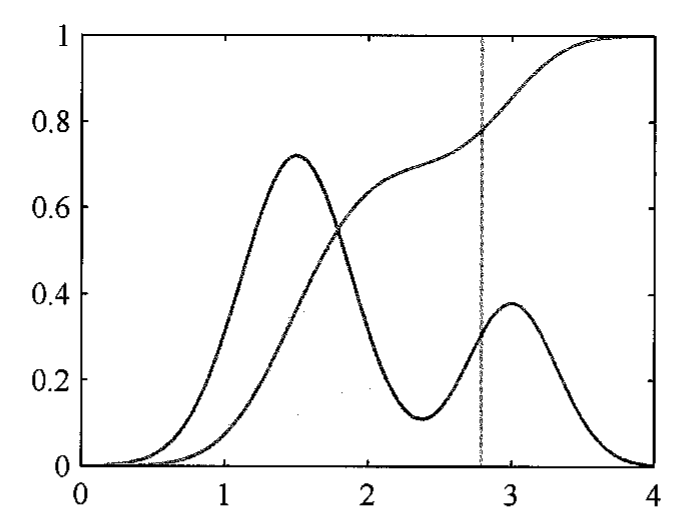
\includegraphics[width=0.5\textwidth]{ch05-fig5-17-probit-threshold.png}
  \caption{蓝色曲线所示为概率密度$p(\theta)$，在本例中由两个 Gauss 混合分布及其累积分布函数$f(a)$（用红色曲线表示）给出。请注意，蓝色曲线在任何一点的值，例如垂直绿线处的值，对应于红色曲线在同一点的斜率。相反，红色曲线在此点的值对应于绿色阴影区域内蓝色曲线下的面积。在随机阈值模型中，如果$a=\boldsymbol{w}^{\mathsf{T}}\boldsymbol{\phi}$的值超过阈值，则类标签取$t=1$，否则取$t=0$，这等价于由累积分布函数$f(a)$给出的激活函数}
  \label{figure:ch05-噪声阈值}
\end{figure}

举个具体的例子，假设密度$p(\theta)$由一个零均值、单位方差的 Gauss 分布给出。相应的累积分布函数为

\begin{align}
  \Phi(a)=\int_{-\infty}^{a}\mathcal{N}(\theta\mid 0,1)\,\mathrm{d}\theta
  \label{align:ch05-probit函数}
\end{align}

\begin{definition}[probit 函数与 erf 函数]\label{definition:ch05-probit函数}
\eqref{align:ch05-probit函数}定义的函数$\Phi$称为 probit 函数。函数
\begin{align}
  \operatorname{erf}(a)=\frac{2}{\sqrt{\pi}}\int_{0}^{a}\exp\left(-\theta^{2}/2\right)\mathrm{d}\theta
  \label{align:ch05-erf函数}
\end{align}
称为 erf 函数。
\end{definition}

注意，使用具有一般均值和方差的 Gauss 分布并不会改变模型，因为这等同于重新缩放线性系数$\boldsymbol{w}$。许多数值计算程序库都支持计算\eqref{align:ch05-erf函数}中的 erf 函数，它与 probit 函数的关系如下（见\cref{exercise:ch05-23}）：

\begin{align}
  \Phi(a)=\frac{1}{2}\left\{1+\frac{1}{\sqrt{2}}\operatorname{erf}(a)\right\}
  \label{align:ch05-probit-erf}
\end{align}

\begin{proposition}[probit 函数与 erf 函数的关系]\label{proposition:ch05-probit与erf}
设$\Phi$与$\operatorname{erf}$分别由\eqref{align:ch05-probit函数}与\eqref{align:ch05-erf函数}定义，则\eqref{align:ch05-probit-erf}成立。
\end{proposition}

\begin{proof}
（重构新增）记$I(a)=\int_0^a e^{-\theta^{2}/2}\,\mathrm{d}\theta$。由$\mathcal{N}(\theta\mid0,1)=e^{-\theta^{2}/2}/\sqrt{2\pi}$与$\Phi(0)=1/2$，
\begin{align}
  \Phi(a)=\frac{1}{2}+\frac{1}{\sqrt{2\pi}}I(a)
\end{align}
而由\eqref{align:ch05-erf函数}，$\operatorname{erf}(a)=\frac{2}{\sqrt{\pi}}I(a)$，故$I(a)=\frac{\sqrt{\pi}}{2}\operatorname{erf}(a)$。代入得
\begin{align}
  \Phi(a)=\frac{1}{2}+\frac{1}{\sqrt{2\pi}}\cdot\frac{\sqrt{\pi}}{2}\operatorname{erf}(a)=\frac{1}{2}+\frac{1}{2\sqrt{2}}\operatorname{erf}(a)=\frac{1}{2}\left\{1+\frac{1}{\sqrt{2}}\operatorname{erf}(a)\right\}
\end{align}
即\eqref{align:ch05-probit-erf}。
\end{proof}

% SUPPLEMENT: parent=definition:ch05-probit函数; kind=motivation; location=紧随其后的 remark（重构新增）
% SUPPLEMENT: parent=proposition:ch05-probit与erf; kind=motivation; location=紧随其后的 remark（重构新增）
\begin{remark}（重构新增）
命题的证明只用到两件事：$\Phi$关于0对称（故$\Phi(0)=1/2$）以及两个积分只相差一个常数因子。\eqref{align:ch05-erf函数}中的因子$1/\sqrt{2}$使$\operatorname{erf}$的自变量按标准差缩放，若改用常见的$\operatorname{erf}(a)=\frac{2}{\sqrt{\pi}}\int_0^{a}e^{-\theta^{2}}\mathrm{d}\theta$，则关系式变为$\Phi(a)=\frac12\{1+\operatorname{erf}(a/\sqrt2)\}$，两者等价但常数位置不同。使用 erf 的实际原因是许多数值库只提供 erf 而无 probit；两者可以互相换算，因此计算上无实质差别。
\end{remark}

基于 probit 函数的广义线性模型称为 probit 回归模型。通过对前面讨论的思路直接进行扩展，我们可以利用最大似然法确定模型的参数。实际上，使用 probit 回归得出的结果往往与使用 logistic 回归得到的结果相似。

\begin{definition}[probit 回归]\label{definition:ch05-probit回归}
若二分类模型的后验概率取$p(C_1\mid\boldsymbol{\phi})=\Phi(\boldsymbol{w}^{\mathsf{T}}\boldsymbol{\phi})$的形式，其中$\Phi$为\eqref{align:ch05-probit函数}定义的 probit 函数，则称该模型为 probit 回归（probit regression）模型。
\end{definition}

% SUPPLEMENT: parent=definition:ch05-probit回归; kind=motivation; location=紧随其后的 remark（重构新增）
\begin{remark}（重构新增）
probit 回归与 logistic 回归同属广义线性模型，区别只在连接函数：probit 用标准正态分布函数，logistic 用 sigmoid。二者的决策面都是超平面，参数个数相同，估计方法也相同（最大似然 + 迭代）。差别体现在尾部：probit 的尾部按$e^{-a^{2}/2}$衰减，logistic 按$e^{-a}$衰减，因此远离决策面的点对 probit 的似然贡献更小，probit 对离群值更敏感（见\cref{proposition:ch05-尾部衰减}）。在实际数据上，两者的预测往往非常接近，因为两条曲线在中心区域几乎重合（见\cref{figure:ch05-sigmoid与probit}）。
\end{remark}

实际应用中可能出现的一个问题是离群值。例如，在测量输入向量$\boldsymbol{x}$时出现的误差或对目标值$t$的错误标记，都可能导致离群值的出现。因为这些点可能离理想的决策边界很远，它们会严重扭曲分类器。logistic 回归模型和 probit 回归模型在这方面的表现不同，因为在$|x|\to\infty$的情况下，logistic sigmoid 函数的尾部衰减为$\exp(-x)$，而 probit 函数的尾部衰减为$\exp(-x^{2})$，因此 probit 模型对离群值更为敏感。

\begin{proposition}[尾部衰减的比较]\label{proposition:ch05-尾部衰减}
对$a>0$，有
\begin{align}
  \sigma(-a)=\frac{e^{-a}}{1+e^{-a}},\qquad \frac{e^{-a}}{2}\leqslant\sigma(-a)\leqslant e^{-a},
\end{align}
而对 probit 函数有
\begin{align}
  1-\Phi(a)=\int_{a}^{\infty}\mathcal{N}(\theta\mid0,1)\,\mathrm{d}\theta\leqslant\frac{1}{a\sqrt{2\pi}}e^{-a^{2}/2}.
\end{align}
因此 logistic 的尾部按$e^{-a}$衰减，probit 的尾部按$e^{-a^{2}/2}$衰减。
\end{proposition}

\begin{proof}
（重构新增）由$\sigma(-a)=1/(1+e^{a})=e^{-a}/(1+e^{-a})$，且$a\geqslant0$时$1\leqslant1+e^{-a}\leqslant2$，得$\frac{e^{-a}}{2}\leqslant\sigma(-a)\leqslant e^{-a}$。对 probit，记$\varphi(\theta)=\mathcal{N}(\theta\mid0,1)$，则$\varphi'(\theta)=-\theta\varphi(\theta)$。当$\theta\geqslant a>0$时$\theta/a\geqslant1$，故
\begin{align}
  1-\Phi(a)=\int_{a}^{\infty}\varphi(\theta)\,\mathrm{d}\theta\leqslant\int_{a}^{\infty}\frac{\theta}{a}\varphi(\theta)\,\mathrm{d}\theta=\frac{1}{a}\int_{a}^{\infty}\theta\varphi(\theta)\,\mathrm{d}\theta=\frac{\varphi(a)}{a}=\frac{1}{a\sqrt{2\pi}}e^{-a^{2}/2}
\end{align}
其中倒数第二个等号用了$-\varphi'=\theta\varphi$，即$\int_a^\infty\theta\varphi(\theta)\mathrm{d}\theta=\varphi(a)$。故 probit 的尾部至多按$e^{-a^{2}/2}$衰减，比$e^{-a}$快得多。
\end{proof}

% SUPPLEMENT: parent=proposition:ch05-尾部衰减; kind=motivation; location=紧随其后的 remark（重构新增）
\begin{remark}（重构新增）
两个尾部估计都是上界，但足以说明量级差别：当$a$从10增到20时，$e^{-a}$缩小约$e^{-10}\approx4.5\times10^{-5}$倍，而$e^{-a^{2}/2}$缩小约$e^{-150}$倍。因此一个远离决策面的离群点对 probit 的似然几乎“不可见”，而对 logistic 仍有非零影响，这就是“probit 对离群值更敏感”的定量含义。注意这里的$a$是带符号的预激活，讨论离群值时应按$|a|$理解；若离群点被正确分类且$a$很大，其似然接近1，对参数的拉动反而小，真正有害的是被错标或位于边界远处的点。
\end{remark}

\subsection{规范连接函数}\label{subsection:ch05-规范连接函数}

对于 Gauss 噪声分布的线性回归模型来说，与负对数似然对应的误差函数就是平方和误差函数（其梯度见\cref{align:ch04-似然梯度}）。如果我们在关于数据点$n$对误差函数的贡献方面对参数向量$\boldsymbol{w}$求导，则得到的形式为“误差”$(y_n-t_n)$乘以$\boldsymbol{\phi}_n$，其中$y_n=\boldsymbol{w}^{\mathsf{T}}\boldsymbol{\phi}_n$。同样，对于 logistic sigmoid 函数与交叉熵误差函数\,[即\eqref{align:ch05-交叉熵}]\,的组合以及 softmax 函数与多类交叉熵误差函数\,[即\eqref{align:ch05-多类交叉熵}]\,的组合，我们也能得到同样的简单形式。需要说明的是，这是假定目标变量的条件分布来自指数族分布以及相应的激活函数选择\,[即规范连接函数（canonical link function）]\,的一般结果。

让我们再次使用指数族分布的限制形式（其一般形式见\cref{align:ch03-指数族定义}）。请注意，这里我们对目标变量$t$采用了指数族分布假设，而在\cref{subsection:ch05-指数族分布}中，我们对输入向量$\boldsymbol{x}$采用了指数族分布假设。因此，考虑目标变量的条件分布，其形式为

\begin{align}
  p(t\mid\eta,s)=\frac{1}{s}h\left(\frac{t}{s}\right)g(\eta)\exp\left\{\frac{\eta t}{s}\right\}
  \label{align:ch05-指数族目标}
\end{align}

利用推导\cref{align:ch03-指数族矩}时的相同论证思路，我们可以看到，$t$的条件均值（用$y$表示）由下式给出：

\begin{align}
  y=\mathbb{E}[t\mid\eta]=-s\frac{\mathrm{d}}{\mathrm{d}\eta}\ln g(\eta)
  \label{align:ch05-条件均值}
\end{align}

因此，$y$和$\eta$必须相关，它们之间的关系为$\eta=\psi(y)$。

根据 Nelder and Wedderburn（1972），我们将广义线性模型定义为$y$是输入（或特征）变量线性组合的非线性函数的模型，从而有

\begin{align}
  y=f\left(\boldsymbol{w}^{\mathsf{T}}\boldsymbol{\phi}\right)
  \label{align:ch05-广义线性}
\end{align}

其中$f(\cdot)$在机器学习文献中称为激活函数，而$f^{-1}(\cdot)$在统计学中称为连接函数。

\begin{definition}[规范连接函数]\label{definition:ch05-规范连接函数}
设目标变量$t$的条件分布为\eqref{align:ch05-指数族目标}，$y=\mathbb{E}[t\mid\eta]$由\eqref{align:ch05-条件均值}给出，$\psi$为$\eta=\psi(y)$所定义的关系。若连接函数取$f^{-1}(y)=\psi(y)$，即使得线性预激活$a=\boldsymbol{w}^{\mathsf{T}}\boldsymbol{\phi}$恰等于自然参数$\eta$，则称该连接函数为规范连接函数（canonical link function）。
\end{definition}

% SUPPLEMENT: parent=definition:ch05-规范连接函数; kind=motivation; location=紧随其后的 remark（重构新增）
\begin{remark}（重构新增）
规范连接的含义是“让线性预激活直接等于自然参数”，从而使对数似然对参数的导数中不出现额外的链式因子（见\cref{proposition:ch05-规范连接梯度}）。它不是唯一的选择，但在给定噪声分布时是使推导最简洁的选择，因此称为“规范”。对 Bernoulli 分布，$\eta=\ln[\mu/(1-\mu)]$即 logit，故 logistic 回归使用规范连接；对 Gauss 分布，$\eta=\mu$，故线性回归使用恒等连接；对 Poisson 分布，$\eta=\ln\mu$。注意这里的“分布”是对目标变量$t$的假设，而不是对输入$\boldsymbol{x}$的假设，这与\cref{subsection:ch05-指数族分布}的生成式视角不同。
\end{remark}

考虑该模型的对数似然函数，作为$\eta$的函数，其计算公式为

\begin{align}
  \ln p(\boldsymbol{t}\mid\eta,s)=\sum_{n=1}^{N}\ln p(t_n\mid\eta_n,s)=\sum_{n=1}^{N}\left\{\ln g(\eta_n)+\frac{\eta_nt_n}{s}\right\}+\text{const}
  \label{align:ch05-对数似然}
\end{align}

其中，我们假设所有观测值都有一个共同的尺度参数（相当于 Gauss 分布的噪声方差），因此$s$与$n$无关。对数似然关于模型参数$\boldsymbol{w}$的导数为

\begin{align}
  \nabla_{\boldsymbol{w}}\ln p(\boldsymbol{t}\mid\eta,s)&=\sum_{n=1}^{N}\left\{\frac{\mathrm{d}}{\mathrm{d}\eta_n}\ln g(\eta_n)+\frac{t_n}{s}\right\}\frac{\mathrm{d}\eta_n}{\mathrm{d}y_n}\frac{\mathrm{d}y_n}{\mathrm{d}a_n}\nabla_{\boldsymbol{w}}a_n\nonumber\\
  &=\sum_{n=1}^{N}\frac{1}{s}\left\{t_n-y_n\right\}\psi'(y_n)f'(a_n)\boldsymbol{\phi}_n
  \label{align:ch05-梯度链式}
\end{align}

其中$a_n=\boldsymbol{w}^{\mathsf{T}}\boldsymbol{\phi}_n$，我们使用了$y_n=f(a_n)$和$\mathbb{E}[t\mid\eta]$的结果\eqref{align:ch05-条件均值}。可以看到，如果我们为连接函数$f^{-1}(y)$选择一种特殊的形式，就可以极大地简化计算过程。

\begin{align}
  f^{-1}(y)=\psi(y)
  \label{align:ch05-规范连接条件}
\end{align}

由于$f(\psi(y))=y$，因此$f'(\psi)\psi'(y)=1$。同样，由于$a=f^{-1}(y)$，得出$a=\psi$，因此$f'(a)\psi'(y)=1$。在这种情况下，误差函数的梯度减小为

\begin{align}
  \nabla\ln E(\boldsymbol{w})=\frac{1}{s}\sum_{n=1}^{N}\left\{y_n-t_n\right\}\boldsymbol{\phi}_n
  \label{align:ch05-规范连接梯度}
\end{align}

\begin{proposition}[规范连接下的梯度化简]\label{proposition:ch05-规范连接梯度}
设目标变量的条件分布为\eqref{align:ch05-指数族目标}，模型为\eqref{align:ch05-广义线性}，且连接函数为规范连接，即$f^{-1}=\psi$。则对数似然关于$\boldsymbol{w}$的梯度为
\begin{align}
  \nabla_{\boldsymbol{w}}\ln p(\boldsymbol{t}\mid\eta,s)=\frac{1}{s}\sum_{n=1}^{N}\left(t_n-y_n\right)\boldsymbol{\phi}_n.
\end{align}
\end{proposition}

\begin{proof}
（重构新增）由\eqref{align:ch05-条件均值}，$\dfrac{\mathrm{d}}{\mathrm{d}\eta_n}\ln g(\eta_n)=-\dfrac{y_n}{s}$。代入\eqref{align:ch05-梯度链式}的第一个等号，括号内变为$(t_n-y_n)/s$。在规范连接下$a_n=\eta_n=\psi(y_n)$，故$\psi'(y_n)f'(a_n)=1$。于是\eqref{align:ch05-梯度链式}化为$\dfrac{1}{s}\sum_n(t_n-y_n)\boldsymbol{\phi}_n$。
\end{proof}

% SUPPLEMENT: parent=proposition:ch05-规范连接梯度; kind=motivation; location=紧随其后的 remark（重构新增）
\begin{remark}（重构新增）
命题说明了“规范连接”这一名称的由来：正是它使链式因子$\psi'(y)f'(a)$恒等于1，从而梯度只剩“误差乘特征”。三个特例：Gauss + 恒等连接给出线性回归的平方和梯度；Bernoulli + logit 给出\eqref{align:ch05-交叉熵梯度式}；多项分布 + softmax 给出\eqref{align:ch05-多类梯度式}。关于原书\eqref{align:ch05-规范连接梯度}的写法，需要说明两点：其一，按\eqref{align:ch05-梯度链式}，对数似然的梯度应为$\frac{1}{s}\sum_n(t_n-y_n)\boldsymbol{\phi}_n$，而\eqref{align:ch05-规范连接梯度}印为$\{y_n-t_n\}$，两者相差一个符号；其二，左端的记号“$\nabla\ln E(\boldsymbol{w})$”应为$\nabla_{\boldsymbol{w}}\ln p$或负对数似然的梯度$\nabla E$，因为$E$本身已是对数似然的负值。若取$E$为负对数似然，则$\nabla E=\frac{1}{s}\sum_n(y_n-t_n)\boldsymbol{\phi}_n$，与印出的右端一致。因此这里按原书照译，同时指出其符号与记号的确切含义，以免读者在推导中混淆。
\end{remark}

我们已经看到，误差函数的选择与输出-单元激活函数的选择之间存在自然的配对。尽管我们是在单层网络的背景下推导出这一结果的，但同样的考虑因素也适用于后续章节讨论的深度神经网络。

\end{document}
